\section{Clustering: K-Means}
% Genaue Betrachtung des K-Means wurde gestartet, die Beispiele müssen herauskommen, und in Beispiel Skripte überführt werden.

\subsection{Introduction}
\begin{itemize}
	\item Die Grundidee ist, einen Datensatz in $k$ Partitionen zu teilen, sodass die Summe der quadrierten Abweichungen von den Cluster-Schwerpunkten minimal ist.
	\begin{align}
		J = \sum_{i=1}^{k}\sum_{x_j\in S_i} \left| \left| x_j - \mu_i \right| \right|^2  
	\end{align}
	mit den Datenpunkten $x_j$ und den Schwerpunkten $\mu_i$ der Cluster $S_i$.
	\item Man spricht von \textit{Clustering durch Varianzminimierung}.
	\item Der Ausdruck $\left| \left| x_i -\mu_i \right| \right|^2$ beschreibt die Euklidische Distanz zwischen dem Datenpunkt und dem Schwerpunkt $\mu_i$ des jeweiligen Clusters $S_i$.
	\item Zum Anfang werden $k$ Cluster ausgewählt.
	\item Das Ziel ist, dass jedes Objekt am Ende einem Clusterschwerpunkt zugewiesen wird.
	\item Schwachstellen des Algorithmus ist, dass die mehrere Lösungen gefunden werden können. Diese hängen von der Wahl der Startpunkt für $\mu_i$ ab. \\
	
	Es gibt verschiedene Algorithmen die die Möglichkeit anbieten, mehrere Iterationen durchzuführen, mit verschiedenen Startwerten.
	\item Eine weitere Schwachstelle ist, dass die Anzahl von $k$ am Anfang festgelegt werden muss. Welches $k$ das richtig ist, kann somit nach den jeweiligen Iterationen passieren.
	\item Für beide Schwachstellen hilft der \textit{Silhouttenkoeffizient}.
	\item Der Algorithmus sucht stets nach konvexen Clustern. Andere Algorithmen können auch andere anders geformte, dichtebasisierte Cluster finden, z. B. \textit{DBSCAN}.
	\item Weil der Algorithmus jeden Punkt einem Cluster zuweist, können Außreißer das Ergebnis verfälschen. Eine \textit{Noisereduction} ist vorher durchzuführen oder andere Algorithem auszuwählen.
\end{itemize}

\subsection{Silhoutte}
Eine Silhoutten gibt Auskunft, wie gut die Zuordnung einer Beobachtung $o$ zu den nächstgelegenen Clustern $A$ und $B$.\\

Darauf aufbauend ist der \textit{Silhouttenkoeffizent}. Dies ist eine Maßzahl für die Qualität der Cluster unabhängig deren Anzahl.

\paragraph{Silhoutte}
Gehört $o$ zum Cluster $A$, so ist die \textit{Silhoutte} von $o$ definiert als: 
\begin{align}
	S(o)= \begin{cases}
		0 & \text{, wenn $o$ einziges Element von $A$ ist} \\
		\dfrac{dist(B,o) - dist(A,0)}{\max\left\lbrace dist(B,o),dist(A,o)\right\rbrace} & \text{, sonst}
	\end{cases}
\end{align}

Die Distanz zwischen dem Objekt $o$ und dem Cluster $A$ sowie $B$ wird durch die maximale Distanz. Daraus folgt, dass $S(o)$ zwischen $-1$ und $1$ liegt.

\begin{itemize}
	\item $S(o) < 0$, dann gehört das Objekt zum nächstgelegenen Cluster $B$. - Das Cluster kann verbessert werden oder Außreißer entfernt.
	\item $S(o) \approx 0$, dann liegt das Objekt zwischen beiden Clustern.
	\item $S(o) \approx 1$, dann liegt das Objekt im richtigen Cluster.
\end{itemize}

Die Berechnung der Distanz zwischen dem Objekt $o$ und dem Cluster $A$ erfolgt wie:
\begin{align}
	dist(A,o) = \frac{1}{n_A - 1}\sum_{a\in A, a \neq o} dist(a,o)
\end{align}
als der Mittelwert der Distanz zwischen \textit{allen anderen Objekten} im Cluster $A$ und dem Objekt $o$. Die Anzahl der Objekte im Cluster $A$ wird mit $n_A$ definiert.\\

Analog wird die Distanz zum nächstgelegenen Cluster $B$ berechnet als die minimale durchschnittliche Distanz
\begin{align}
	dist(B,o) = \min_{C\neq A} \underbrace{\left(\frac{1}{n_c} \sum_{c\in C}dis(C,o)\right)}_{=dist(C,o)}
\end{align}
Dabei wird für alle Cluster, die das Objekt $o$ nicht enthalten\footnote{Weil $o$ in $A$ liegt.} die Distanz $dist(C,o)$ berechnet. Der nächstgelegene Cluster ist der mit der kleinsten Distanz.

\paragraph{Silhouettenkoeffizient}
Der Silhouttenkoeffizient ist definiert als 
\begin{align}
	s_C = \frac{1}{n_C}\sum_{o\in C}S(o)
\end{align}
arithmetisches Mittle aller $n_C$ Silhoutten eines Clusters $C$.
Diese Koeffizient kann für jeden Cluster oder den gesamten Datensatz berechnet werden.

\subsection{Test Data Sets}
Neue Algorithmen können problemlos arbeiten, diese zu testen, ob sie das tun, was sie tun sollen, ist nicht immer erkennbar. \\

Dafür hat \textit{scikit} Datensatz Pakete. Diese ermöglichen spezifischen Datensätze zu generieren, die 
\begin{itemize}
	\item in ihren Hyperparameter angepasst werden
	\item und skalierbar sind.
\end{itemize}

Im folgenden sollen drei Problem von \textit{Klassifikation} aufgegriffen. Dabei beschreibt \textit{Klassifikation}, dass einem Teilmengen eines Datensatzes \textit{Labels} zu gewissen werden. 

\begin{figure}[H]
	\centering
	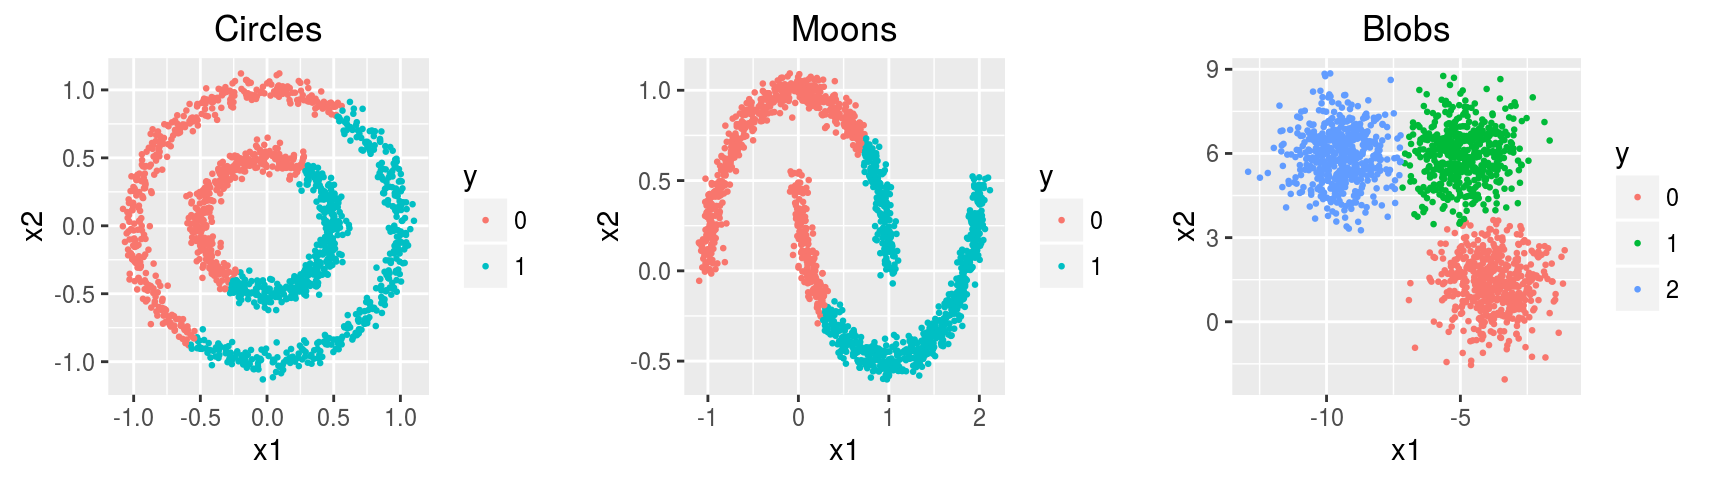
\includegraphics[scale = 0.8]{attachment/chapter_1/Scc160}
	\caption{Blobs, Moons, Circles}
\end{figure} 


\subsection{Blobs Classification Problem}
Die Funktion $make\_ blobs()$ generiert einen Datensatz, welcher $n$ Cluster beinhaltet. Dabei werden die Cluster zufällig gesetzt und die Datenpunkte um die Zentren normalverteilt. Die unabhängigen Dimensionen, oder auch \textit{Features} genannt, können ebenso bestimmt werden. Eine Visualisierung von zwei bis drei Features ist nur möglich. Die Labels werden ebenfalls als zweiter Output mit ausgegeben.
\begin{lstlisting}[style=Python]
	# Generate classification dataset
	X, labels = make_blobs(
	n_samples=100, #n-datapoints equalie devided amoung the centers
	centers=2, #centers in the dataset
	n_features=2 #columns return
	)
\end{lstlisting}

Im Folgenden wird eine Größe der \textit{Features} höher 2 nicht betrachtet, weil der Plot auf 2D ausgelegt ist.
\begin{figure}[H]
	\centering
	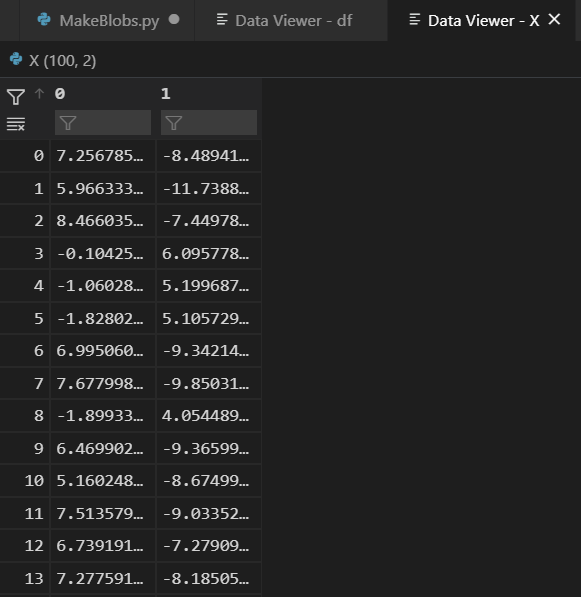
\includegraphics[scale = 0.8]{attachment/chapter_1/Scc161}
	\caption{Die Variable $X$ sieht mit $n_features = 2$ wie folgt aus}
\end{figure}

\begin{figure}[H]
	\centering
	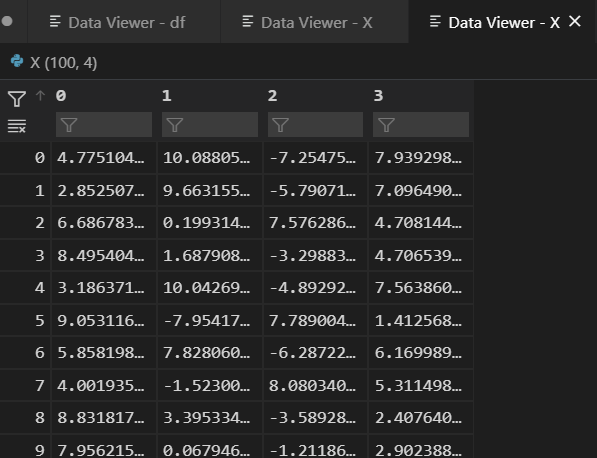
\includegraphics[scale = 0.8]{attachment/chapter_1/Scc162}
	\caption{Die Variable $X$ sieht mit $n_features = 4$ wie folgt aus}
\end{figure}

Der Testdatensatz ist somit erstellt. Für die Plotung wird diese im Folgenden vorbereitet.
\begin{lstlisting}[style=Python]
	# Collect all in one df
	df = Dataframe(dict(x = X[:;0],y = X[:;1], label = y))
\end{lstlisting}\footnote{\textit{class pandas.DataFrame(data=None, index=None, columns=None, dtype=None, copy=False)}
	\begin{itemize}
		\item \textbf{data} ndarray (structured or homogeneous), Iterable, dict, or DataFrame\\
		Dict can contain Series, arrays, constants, dataclass or list-like objects. If data is a dict, column order follows insertion-order.
		\item \textbf{index} $\dots$
\end{itemize}} \footnote{$X[:;0]$ bedeutet, dass alle Zeile $:$ und die erste Spalte mit Index $0$ ausgewählt wird.}
\footnote{Die Funktion \textit{dict()} ließt drei Werte ein $x$, $y$ und $label$. Die Auslesung erfolgt über die Ausgabe von $X$ und $y$. Dabei wird $X[\textit{Zeile},\textit{Spalte}]$ angewandt, um die entsprechenden Werte auszulesen. Bsp.: $X[1;1] >>> -8,2313234234$
}

Für die unterschiedlichen Labels werden eine \textit{Series} erstellt, welche verschiedenen Farben für die verschiedenen Clusters.

Für die grafische Bewertung wird eine Farbpalette zusammengestellt.
\begin{lstlisting}[style=Python]
	# scatter plot, dots colored by class value
	colors = {0:'red', 1:'blue', 2:'green',3:'yellow'}
\end{lstlisting}
